% AMLBT project report, written to the structure of the instructor's template
% (project/main.tex holds the template itself and is left unedited).
\documentclass[conference]{IEEEtran}
\IEEEoverridecommandlockouts

\usepackage{amsmath,amsfonts}
\usepackage{graphicx}
\usepackage{booktabs}
\usepackage{hyperref}
\usepackage{cite}
\usepackage{xcolor}

\newcommand{\rs}{Rs.\,}

\bibliographystyle{IEEEtran}

\begin{document}

\title{Who Needs a Savings Nudge? Leakage-Free Prediction of\\Household Savings Adequacy in India}

\author{
    \IEEEauthorblockN{Rishabh Agrawal, Prisha Kothari, Akshit Kashyap}
    \IEEEauthorblockA{Goa Institute of Management\\
    Big Data Analytics\\
    Student IDs: \{B2025100, B2026092, B2026059\}\\
    Email: \{rishabh.agrawal25b, prisha.kothari2026b, akshit.kashyap2026b\}@gim.ac.in}
}

\date{\today}

\maketitle

\begin{abstract}
A savings-product or financial-inclusion team cannot review tens of thousands of households by hand to decide who needs support, so the triage has to be automated. We study that triage on the India Human Development Survey-II (41,518 households, 2011--12), predicting whether a household retains at least 20\% of its annual income after recorded consumption. The target is an exact accounting identity over the expense columns, which rules out the obvious feature set: expense-to-income ratios reconstruct the label with 99.75\% agreement, and so do the raw rupee categories. We instead represent spending as each category's share of total expenditure, a vector that sums to one for every household and so carries no information about consumption relative to income. On 28 leakage-free features, XGBoost reaches cross-validated macro-F1 0.837 and ROC-AUC 0.931, confirmed once on a held-out fifth of the sample at 0.838. The margin that matters is much smaller: a single threshold on income already reaches macro-F1 0.743, and at a 25\% contact budget the model reaches 36.6\% of at-risk households against 35.0\% for that rule. SHAP attributes 38.4\% of the model's behaviour to income and 41.9\% to interactions, and shows that a food-dominated budget predicts adequacy once income is controlled, reversing the unconditional reading. Clustering on an isometric log-ratio basis recovers three spending patterns whose association with the outcome nearly doubles when income is held constant. For 71.5\% of at-risk households the gap is too large to close by matching same-income peers, so a budgeting product cannot help them.
\end{abstract}

\begin{IEEEkeywords}
Machine learning, financial inclusion, household survey data, data leakage, compositional data, explainable AI, customer segmentation
\end{IEEEkeywords}

\section{Introduction}

Savings products in India are sold into a population that is mostly not saving. Outreach is expensive per contact, budgets are fixed, and a team that wants to prioritise households by need has no way to inspect tens of thousands of them individually. The decision is a triage: treat this household as on track or at risk, and spend the next contact accordingly.

We frame that triage as binary classification on the India Human Development Survey-II (IHDS-II), a nationally representative survey of 42,152 Indian households conducted in 2011--12 \cite{ihds2}. IHDS-II is unusual among Indian surveys in recording income and category-level expenditure for the same household; the NSS-lineage consumption surveys collect one without the other. After dropping 634 households with non-positive income or missing consumption, 41,518 remain.

The problem is constrained in a way that is easy to miss. A household is labelled on track when it retains at least 20\% of its annual income, and that label is an exact arithmetic function of income and the expense columns. A feature set built from expense-to-income ratios, the intuitive representation, therefore reconstructs the answer instead of predicting it, at 99.75\% agreement when we measured it. The composition shares we use instead describe only the shape of a budget, not its size relative to income.

The second constraint is on reporting. Against a majority-class baseline the model looks excellent; against the rule a team would use in its absence, contact the poorest first, most of the apparent gain disappears. We report both and organise the paper around the second.

\subsection{Scope and objectives}

The project has four objectives: establish by measurement which representations of household spending can legitimately serve as features for a savings-adequacy target; compare seven model families under a validation scheme fixed in advance and quantify the gain over a single-variable rule rather than over chance; explain the winning model with exact tree SHAP values and segment households using a metric that is well defined on the simplex; and translate the results into targeting recommendations that state where the model fails, not only where it works.

\section{Related Work}
\label{sec:related_work}

Predicting household welfare from survey covariates is the core of proxy means testing, the standard method for targeting transfers when income is unobservable. Brown, Ravallion and van de Walle evaluated such tests across nine African countries and found that they miss a large share of the poorest households even when the underlying regression fits well \cite{brown2018}, which is the closest antecedent to our own finding that a good score does not imply a useful targeting instrument. McBride and Nichols showed that out-of-sample validation and machine learning improve on the regression practice then in use \cite{mcbride2018}, and where survey data is unavailable poverty has been predicted from mobile phone metadata \cite{blumenstock2015}. Our task differs in what is predicted and from what: the outcome is a savings residual rather than a consumption level, and the features are the household's own spending composition rather than external proxies for wealth.

Ours is a prediction policy problem in the sense of Kleinberg et al. \cite{kleinberg2015}: we do not claim that contacting a household changes its savings rate, only that ranking by predicted risk allocates a fixed budget better than not ranking. The intervention literature supplies the reason such a ranking is worth having, since simple reminders raise savings measurably \cite{karlan2016}, while Dupas and Robinson show that access constraints rather than preferences explain much of the shortfall among poor households \cite{dupas2013}.

Two measurement results bear on the data. Deaton and Kozel document the divergence between income and consumption aggregates in Indian surveys \cite{deaton2005}, which we inherit as 55.9\% of households reporting consumption above income. Engel's law, food's budget share falling as income rises, appears here unprompted at $r = -0.266$ and inverts once income is conditioned on.

On method we use gradient-boosted trees \cite{chen2016} with SHAP attributions from the exact tree algorithm \cite{lundberg2017,lundberg2020}. Because the eleven spending shares are a composition, we follow Aitchison's treatment of the simplex \cite{aitchison1982}, cluster on an isometric log-ratio basis \cite{egozcue2003} rather than a centred one, which is singular by construction, and replace zeros multiplicatively \cite{martinfernandez2003}. Cluster count is chosen by silhouette score \cite{rousseeuw1987}.

\section{Methodology}

\subsection{Data and target}

The analysis file is built from ICPSR study 36151, dataset DS0002 (Household). IHDS-II records consumption in 52 items under two recall windows, 30-day and annual, so the build annualises as $12 \times \text{monthly} + \text{annual}$ and validates the result against the survey's own aggregate \texttt{COTOTAL}: correlation 0.9931, median difference zero, 97.7\% within 1\%. Items are mapped onto 11 expense categories from the codebook, and occupation is derived as the worker type contributing the most workers, which IHDS does not record directly.

The target is
\begin{equation}
    \texttt{Goal\_Met} = \mathbf{1}\left[\frac{\texttt{INCOME} - \texttt{COTOTAL}}{\texttt{INCOME}} \geq 0.20\right],
    \label{eq:target}
\end{equation}
with both quantities in annual rupees: a household is on track if it retains at least a fifth of its income after all recorded consumption. The rate is 31.93\% positive, a 2.13:1 imbalance, and 30.47\% when survey weights are applied.

Two properties of this definition matter more than the definition itself. The 20\% figure is a convention chosen in advance, not a measurement, so we publish the sensitivity curve: the at-risk share moves from 68.1\% at the benchmark to 61.7\% at 10\% and 74.7\% at 30\%, with about 93.5\% label agreement either way. Every finding below holds across that range; the levels do not. And because IHDS records no savings intention, the benchmark is normative and identical for every household, so the model measures something closer to savings capacity than to goal alignment. No claim here is about goals households set for themselves.

\subsection{The leakage constraint}

Equation~\eqref{eq:target} is an accounting identity, verified on the built data to a maximum absolute error of $5.8 \times 10^{-11}$, and three consequences follow that we tested rather than assumed. The 11 raw rupee categories, with income, reconstruct the label at 99.75\% agreement, and expense-to-income ratios give the identical 99.75\% because they are the same quantities divided through by income. Both are excluded. This is a property of any fixed savings benchmark, not of IHDS: when the threshold is a constant, knowing what fraction of income each category consumes is knowing the answer.

Composition shares, each category divided by \emph{total expenditure}, sum to exactly 1.000000 for every household, so they cannot recover consumption relative to income, and the strongest correlation between any share and the savings rate is 0.056. We report the algebra and the correlation together because a feature can be non-reconstructing and still act as leakage in practice.

Six survey-reported indicators of savings-instrument holding (bank account, fixed deposit, pension or LIC policy, securities, post office account, gold) sit outside the consumption arithmetic, so they are neither features nor leakage. We reserve them as an external check, and they behave as expected: fixed-deposit holding is 15.2\% among on-track households against 8.2\% among the rest.

\subsection{Feature engineering}

Four decisions were settled empirically, and two went against the textbook answer.

Expense-to-income ratios are usually defended as making households comparable across income levels. Tested on a neutral target (\texttt{Has\_Bank\_Savings}, not an accounting function of the expense columns) by fitting on one half of the income distribution and scoring on the other, they transfer \emph{worst}: mean ROC-AUC 0.5893 against 0.6245 for raw rupees and 0.6175 for shares. Dividing by income helps when the raw columns are largely restatements of income, and here they are not, correlating with it at only 0.09--0.43. The division mostly adds noise from a poorly measured denominator, since income is the under-reported side of this survey.

Five categories are zero for more than 30\% of households, so we added binary participation indicators alongside the shares, improving ROC-AUC from 0.9183 to 0.9204. Their univariate effects run in opposite directions: paying any insurance premium is associated with +9.7 points of goal attainment, paying any school fee with $-$8.3 points.

A centred log-ratio transform of the six least zero-inflated shares was proposed, implemented with multiplicative zero replacement, and then rejected at 0.9117 against 0.9212 for the raw shares. It is scale-free within the composition, which discards exactly the level information Engel's law makes predictive, and its basis is singular by construction. We keep it only for the clustering in Section~\ref{sec:personas}, where a metric on the simplex is genuinely needed.

Debt is winsorised at the 99th percentile, a tie broken on interpretability after raw, winsorised and $\log(1+x)$ variants came within 0.0005 ROC-AUC of each other. IHDS records debt as a stock with no repayment instalment, so the feature stands in for a cash-flow burden it cannot directly measure.

The final set is 28 features: 11 composition shares, log income, four household composition variables, highest adult education, five participation indicators, winsorised debt-to-income, a debt indicator and four one-hot categoricals (occupation, area type, caste, religion) with an explicit \texttt{Unknown} level. Missingness is negligible and uninformative: goal attainment among households with missing caste is 0.3176 against 0.3193 among those recording it.

\subsection{Models, validation and metrics}

Seven families were compared: a majority-class baseline, logistic regression, a linear SVM, a decision tree, a random forest, histogram gradient boosting and XGBoost. Kernel SVMs were excluded on cost, scaling roughly quadratically at $n = 41{,}518$. The 20\% test split (8,304 households) is taken in the notebook's first cell, before any model is defined, and evaluated once. Model choice, hyperparameter search and threshold selection all read the 80\% training split under 5-fold stratified cross-validation, with a 15-iteration randomised search over five XGBoost parameters. The linear models use balanced class weights; the boosted models do not need them at 2.13:1.

Macro-F1 is the ranking metric, because the majority baseline scores 0.6807 accuracy while never identifying a single on-track household: accuracy here is gameable by a constant. ROC-AUC is reported alongside it, being threshold-free and so comparable across differently calibrated models. For operational decisions we report precision and recall on \texttt{Goal\_Met} $= 0$, the at-risk class the business acts on, which is not the class a default classification report treats as positive.

\section{Results}

\subsection{What each ingredient is worth}

\begin{figure}[t]
    \centering
    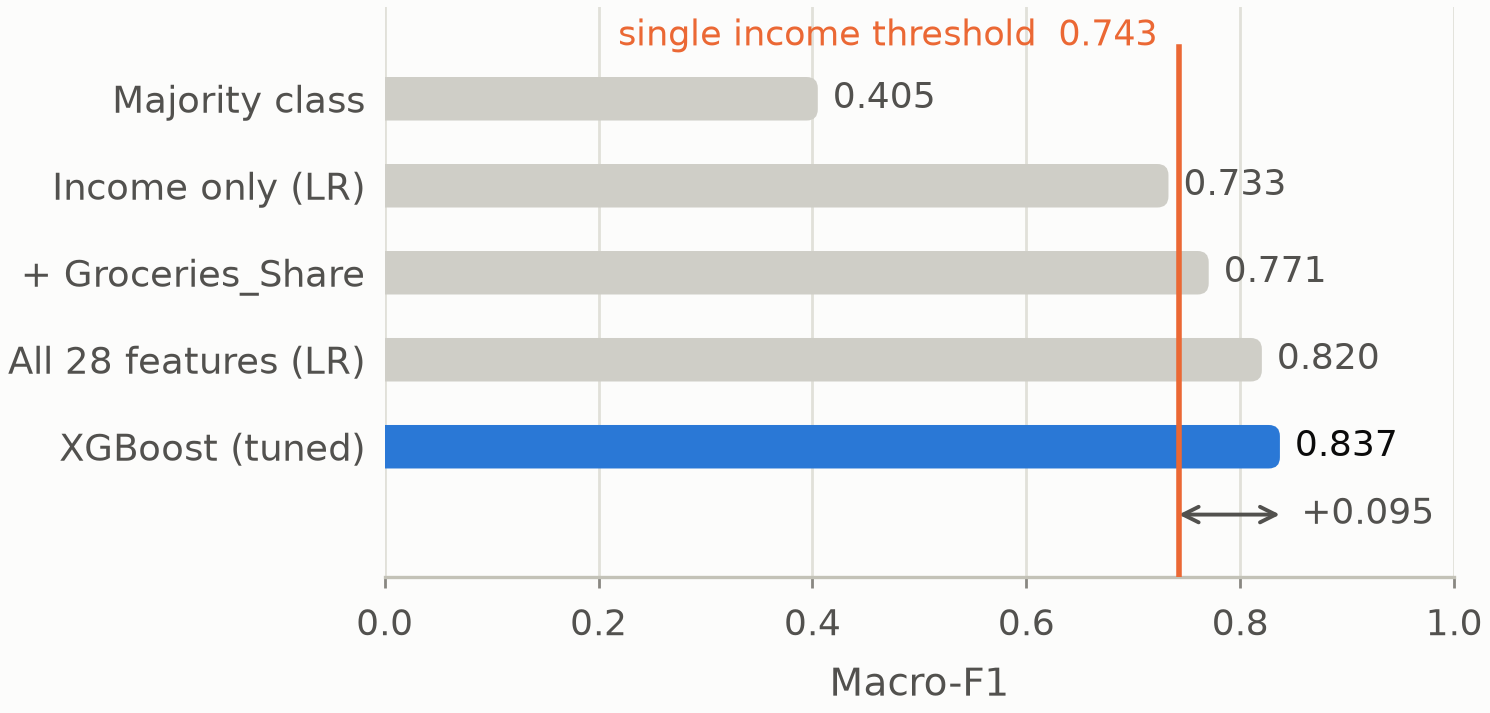
\includegraphics[width=0.93\columnwidth]{figures/fig1_honest_margin.png}
    \caption{Macro-F1 as features and model capacity are added. The vertical line is a depth-1 tree on income alone, which predicts ``on track'' above \rs 121,685 a year. Everything beyond asking how much a household earns is worth 0.095 macro-F1.}
    \label{fig:margin}
\end{figure}

Dummy classifiers fail in different ways: the majority classifier reaches 0.6807 accuracy and 0.4050 macro-F1 with precision and recall of exactly zero on the positive class, while a stratified guesser scores worse on accuracy (0.5649) and better on macro-F1 (0.4948) because it predicts both classes.

The informative baseline is a single threshold. A depth-1 tree on income alone predicts on track above \rs 121,685 a year and reaches 0.7753 accuracy and 0.7425 macro-F1. Adding one spending feature to a logistic model lifts ROC-AUC from 0.8348 to 0.8756, and the full 28-feature set reaches 0.9212 (Fig.~\ref{fig:margin}). Diminishing returns are steep, which correctly predicted that hyperparameter search would not pay: 15 iterations bought 0.0006 macro-F1, about a third of one fold's standard deviation.

\subsection{Model comparison}

\begin{table}[t]
    \centering
    \caption{Five-fold cross-validated performance on the training split. The linear models carry balanced class weights and the boosted models do not, so the threshold-free ROC-AUC column is the fairer comparison between them.}
    \label{tab:models}
    \footnotesize
    \begin{tabular}{l c c c}
        \toprule
        Model & Accuracy & F1 (macro) & ROC-AUC \\
        \midrule
        \textbf{XGBoost} & 0.8614 & \textbf{0.8371} & \textbf{0.9306} \\
        HistGradientBoosting & 0.8606 & 0.8360 & 0.9306 \\
        Random Forest & 0.8512 & 0.8249 & 0.9170 \\
        Logistic Regression & 0.8343 & 0.8186 & 0.9213 \\
        Linear SVM & 0.8332 & 0.8177 & --- \\
        Decision Tree & 0.8067 & 0.7889 & 0.8847 \\
        \midrule
        Single income threshold & 0.7753 & 0.7425 & 0.7438 \\
        Majority class & 0.6807 & 0.4050 & 0.5000 \\
        \bottomrule
    \end{tabular}
\end{table}

XGBoost wins at macro-F1 0.8371 with \texttt{max\_depth}=4, \texttt{learning\_rate}=0.15, \texttt{n\_estimators}=200, \texttt{min\_child\_weight}=5 and \texttt{subsample}=0.9 (Table~\ref{tab:models}). Histogram gradient boosting is 0.0011 behind against a fold-to-fold standard deviation of 0.0018 to 0.0021, so we treat them as tied and select XGBoost on the nominal score. Held-out test macro-F1 is 0.838 on 8,304 households, identical to the cross-validated estimate, with 5,163 of 5,653 at-risk households correctly flagged.

The macro-F1 column understates the linear models: logistic regression and the linear SVM have the highest recall on the on-track class (0.847, 0.848) and the lowest precision, which is balanced class weighting moving the decision boundary rather than a difference in what they learned. On ROC-AUC logistic regression sits at 0.9213 against XGBoost's 0.9306.

For deployment we tune the threshold on the at-risk score rather than accept 0.5. Moving from 80\% to 95\% recall on that class costs 8.5 points of precision (0.941 to 0.856), so even at 95\% recall roughly six of every seven flagged households are genuinely at risk. A missed at-risk household is a silent failure and an unnecessary nudge is cheap, and the trade is favourable here because the at-risk class is the majority.

\subsection{What the model uses}

\begin{figure}[t]
    \centering
    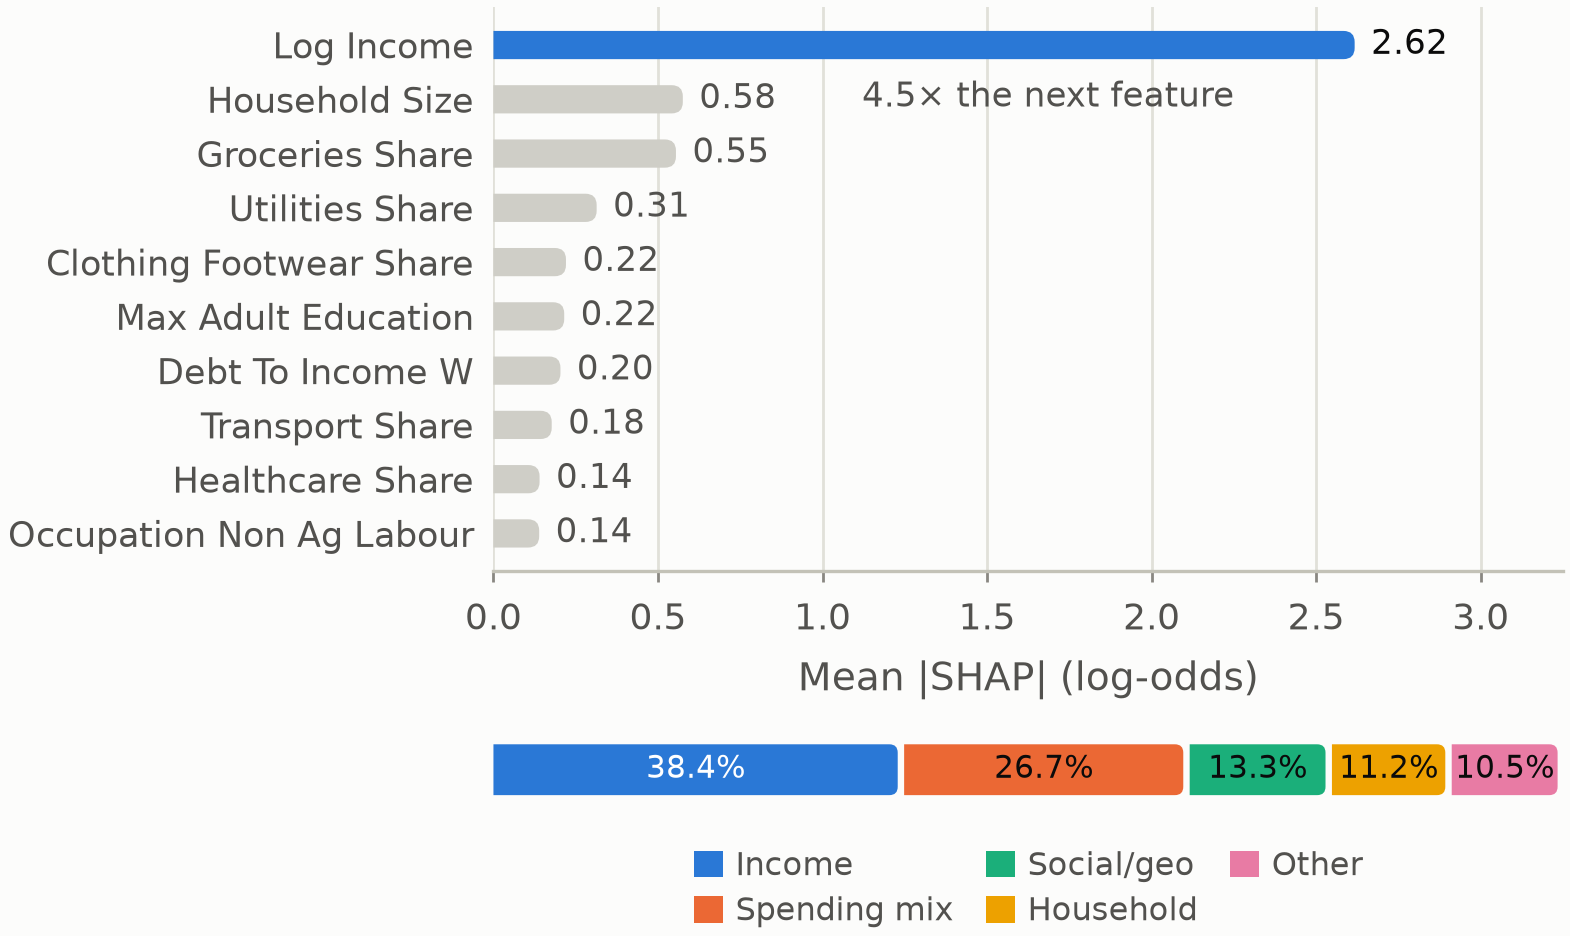
\includegraphics[width=0.93\columnwidth]{figures/fig2_shap.png}
    \caption{Global SHAP attribution for the tuned XGBoost model: the ten largest mean absolute values, and attribution by feature family. ``Social/geo'' is occupation, area type, caste and religion; ``Household'' is size, dependents, dependency ratio and head age; ``Other'' pools participation indicators, debt and education.}
    \label{fig:shap}
\end{figure}

Because the eleven shares sum to one they are exactly singular as a set, so no coefficient on them is identified. Refitting on five disjoint subsamples confirms the symptom: three of eleven share coefficients flip sign against one of five non-compositional controls. Dropping a reference part, the standard remedy, improved median stability by only 1.22 times and made \texttt{Rent\_Share} 17 times \emph{worse}, since rent is zero for 90.4\% of households. We therefore attribute with SHAP on the tree model, which requires no matrix inversion, using XGBoost's own \texttt{pred\_contribs} implementation. Additivity was verified rather than assumed: contributions plus bias reproduce the raw model margin to a maximum absolute error of $8.6 \times 10^{-6}$.

Log income alone carries 38.4\% of total attribution at mean $|$SHAP$|$ 2.617, four and a half times the next feature (Fig.~\ref{fig:shap}). Spending mix accounts for 26.7\%, which is real and second. Interactions are 41.9\% of all attribution and eight of the ten strongest pairs involve income, which is the concrete reason a linear model was not selected: income does not merely add to the prediction, it changes what every spending signal means. A high grocery share means something different at \rs 40,000 of annual income than at \rs 400,000.

The grocery finding reverses the obvious reading, and we record it as a correction rather than as foresight. We captioned the dependence plot from Engel's law, expecting a high food share to push toward ``not on track''. It does the opposite: conditional on income, SHAP for the grocery share runs from about $-3$ at a 10\% food share to about $+1$ at 80\%, crossing zero near 0.45. Once income is in the model the food share is no longer a poverty proxy. What remains is budget shape, and a household whose spending is dominated by food spends proportionally little on the lumpy outlays (health shocks, durables, school fees) that push consumption above income. Reading the conditional model off the unconditional correlation would have produced a backwards recommendation.

Area type behaves the same way. Goal attainment falls monotonically from metro urban (0.4212) to less developed villages (0.2666), but income's SHAP curve is nearly identical across the four types, so the geographic gradient is largely an income gradient wearing a geographic label.

\subsection{Spending personas}
\label{sec:personas}

\begin{figure}[t]
    \centering
    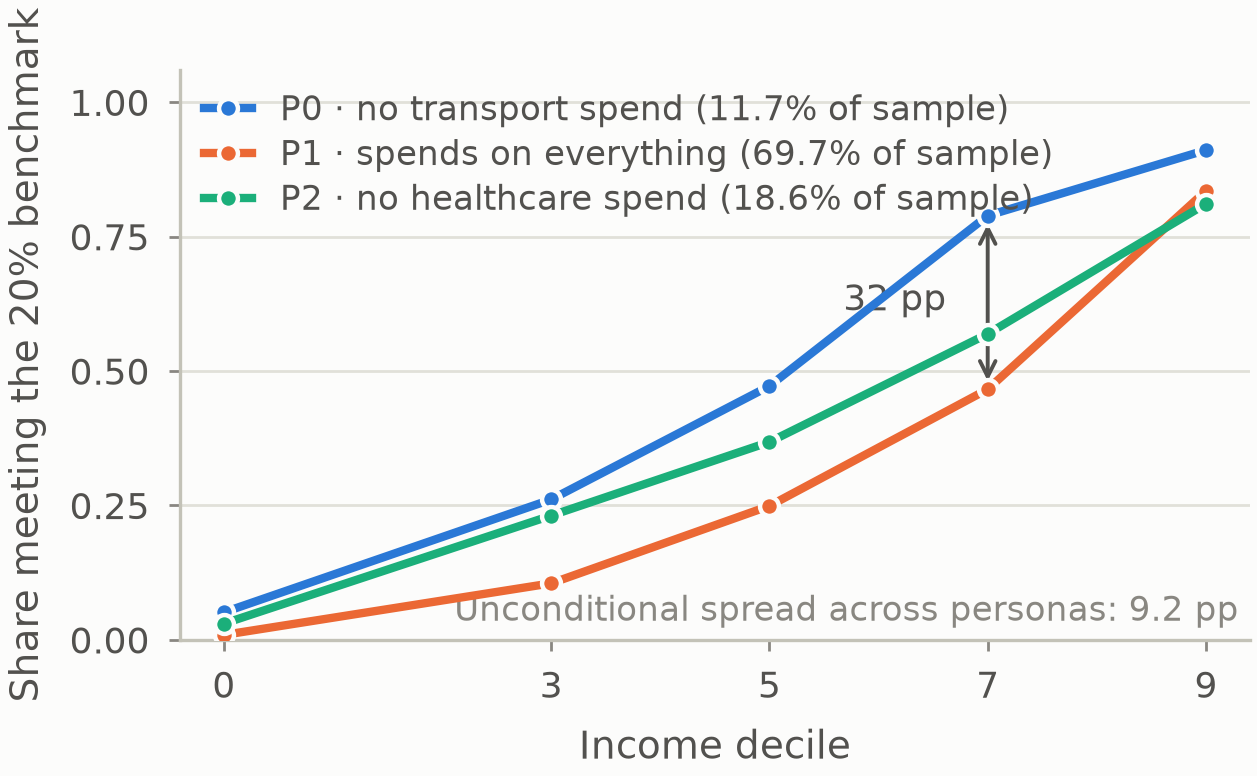
\includegraphics[width=0.93\columnwidth]{figures/fig4_personas.png}
    \caption{Goal attainment by persona within income decile. Unconditionally the personas look nearly unrelated to the outcome (9.2-point spread, Cram\'er's $V = 0.076$); holding income constant, the mean spread rises to 16.7 points and reaches 32 at decile 7.}
    \label{fig:personas}
\end{figure}

\begin{figure*}[t]
    \centering
    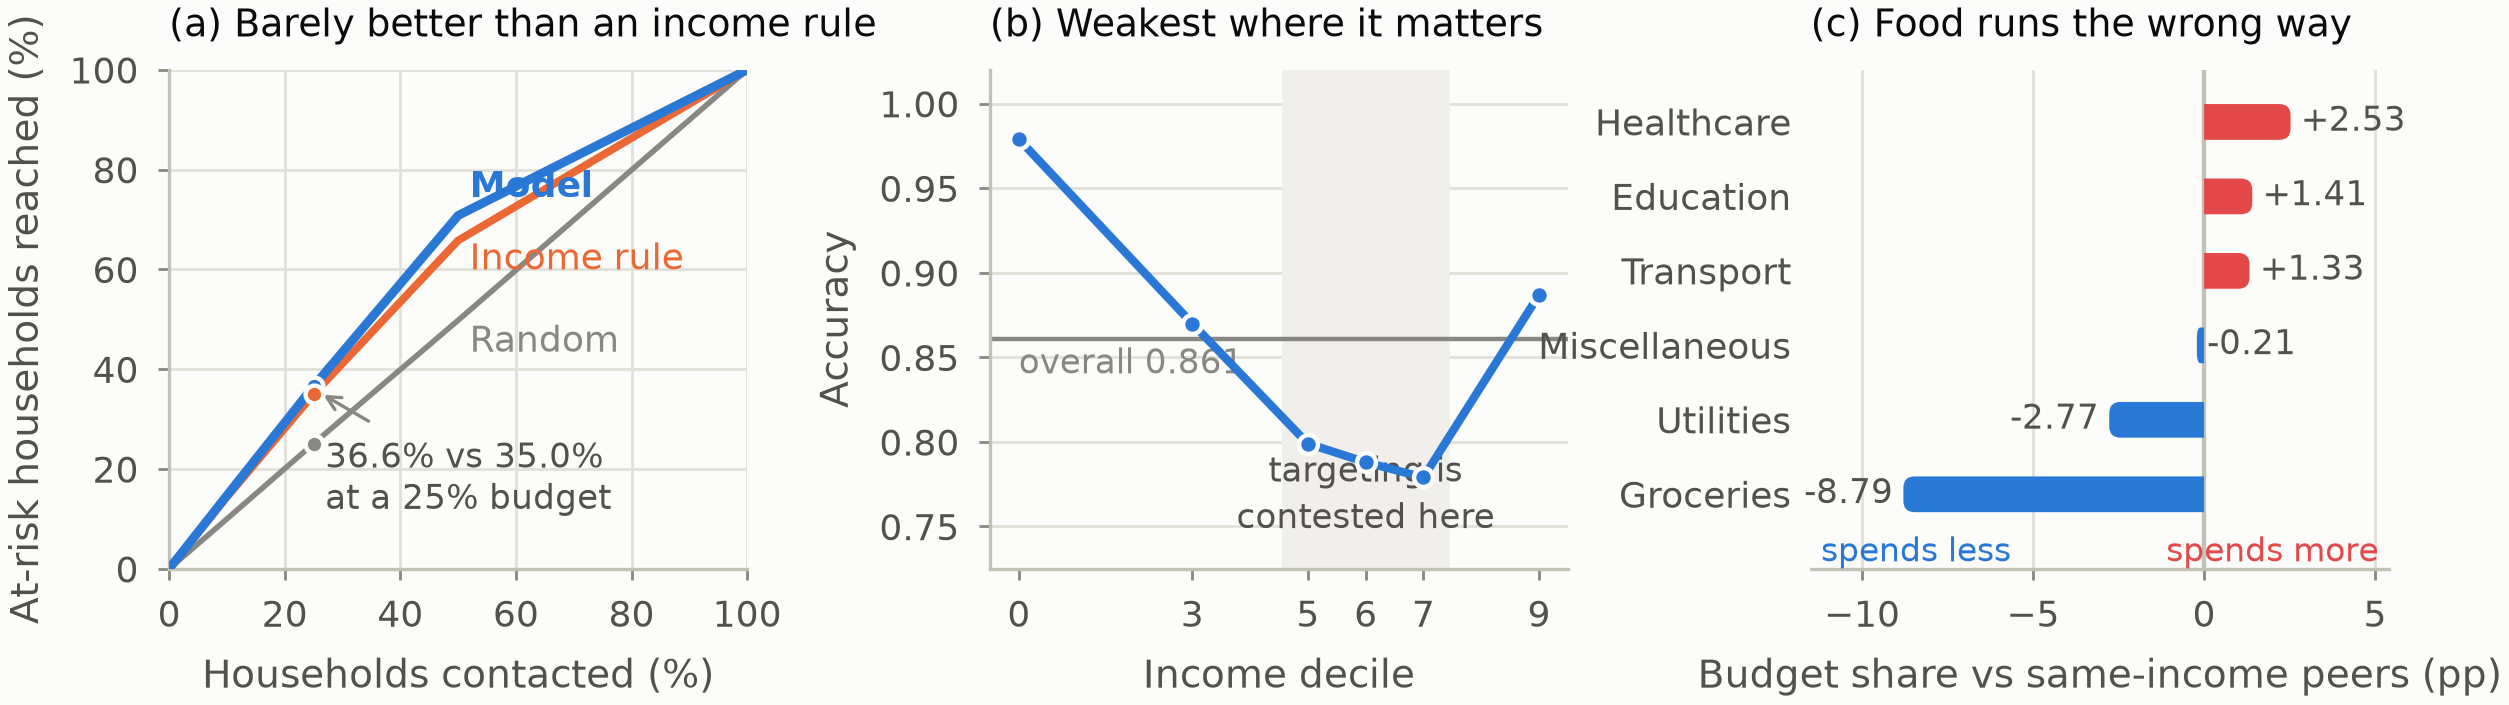
\includegraphics[width=\textwidth]{figures/fig3_business.png}
    \caption{Three views of deployment value. (a) At-risk households reached against contact budget; at a 25\% budget the model's advantage over the income rule is 1.5 percentage points. (b) Accuracy by income decile; the band marks deciles 5 to 7, where at-risk rates run from 70\% to 49\% and targeting is contested. (c) Median budget share of at-risk households against the median on-track household in the same income decile.}
    \label{fig:business}
\end{figure*}

We clustered on a six-part isometric log-ratio basis built from a Helmert contrast matrix, verifying orthonormality to $2.2 \times 10^{-16}$ and that Aitchison distance equals Euclidean distance in the transformed space to $1.8 \times 10^{-15}$. That second check is what makes k-means legitimate here, and it does not hold on raw shares. Silhouette selects $k = 3$ at 0.4115, against 0.2516 for the best raw-share solution.

The clusters are not what the word persona implies. Persona 0 (11.7\% of households) records no transport spend, Persona 2 (18.6\%) records no healthcare spend, and Persona 1 (69.7\%) spends on everything, and the adjusted Rand index between the cluster labels and the raw zero-pattern of the six parts is 0.858. Multiplicative zero replacement gives every transport-less household the same imputed value far out in log-ratio space, so they form a tight, well-separated blob that silhouette rewards. Log-ratio clustering of zero-inflated compositions tends to rediscover the zero pattern like this, and the zero-pattern index is the diagnostic that catches it.

We expected the personas to re-encode income, since income carries more attribution than spending mix. That was falsified twice. The adjusted Rand index between personas and income tertiles is 0.006, so they are close to independent, and income \emph{suppresses} the association with the outcome rather than driving it: the unconditional spread in goal attainment is 9.2 points (Cram\'er's $V = 0.076$) against a mean within-decile spread of 16.7. Fig.~\ref{fig:personas} shows why. Persona 0 has the lowest median income (\rs 48,820) and the highest within-decile attainment, so pooled across incomes its low income cancels its behavioural advantage.

The mechanism is the one behind the grocery result: a household recording no spend in a whole category spends less overall at a given income, so it retains more. Some of that is measurement rather than behaviour, since zero healthcare spend may mean no health event that year. These segments are descriptive, not levers.

\subsection{What the model is worth}

Targeting performance is measured on out-of-fold scores, so no household is ranked by a model that saw it. At a 25\% contact budget the model reaches 36.6\% of at-risk households, the income rule 35.0\% and random contact 25.1\% (Fig.~\ref{fig:business}(a)). The edge over ``contact the poorest first'' is 1.5 percentage points, and we place that number first rather than burying it. Lift over random is 1.46 times, unimpressive by construction, since lift is only large when the target class is rare and here it is 68.1\% of the population. Where the model earns its place is precision: 99.6\% of its top quartile are genuinely at risk against 68.3\% under random contact, a real cut in wasted outreach when cost is per contact.

Reliability degrades where the decision is hardest. Calibration is good, with a maximum absolute error of 0.036 over ten probability bins, so a predicted 70\% means about 70\% and the scores support expected-value arithmetic rather than ranking alone. But accuracy by income decile, Fig.~\ref{fig:business}(b), runs 0.979 in the poorest decile and 0.887 in the richest while falling to 0.779--0.799 in deciles 5 to 7. The extremes need no model: 97.8\% of the poorest decile is at risk and 16.9\% of the richest is. Quoting the overall 0.861 without this breakdown overstates usefulness at the only point where the model changes an action.

To ask which spending is recoverable without assuming what a household could have given up, we benchmark each at-risk household against the median on-track household in the same income decile (Fig.~\ref{fig:business}(c)). Healthcare has the largest median excess at +2.53 points with 63.5\% of at-risk households above their peers, and education is next at +1.41; both are close to non-negotiable, so neither is a legitimate target for a nudge. Miscellaneous spend tops the aggregate table at \rs 36 crore per year, but its median excess is slightly negative, so the aggregate comes from a minority with very large outlays rather than a broad tendency. Groceries runs the wrong way entirely: at-risk households spend 8.8 points \emph{less} of their budget on food than their income peers, and only 27.1\% exceed them.

The largest product implication is the size of the gap. The median at-risk household is \rs 37,114 per year short of the benchmark against \rs 22,939 of peer excess across all categories, and only 28.5\% could reach it even by matching their income peers' spending in every category. A budgeting tool, a round-up feature or a spending nudge all assume the shortfall is behavioural. For roughly seven in ten at-risk households here it is not.

Five recommendations follow: prioritise by income first and use the model to re-rank within income bands; size the campaign as prioritisation rather than needle-finding; treat the shortfall as structural for the 71.5\% who cannot close it through spending; look for a behavioural lever in miscellaneous spend rather than groceries; and report relative priority only, never a prevalence figure.

\section{Discussion}

The headline numbers are good and the honest margin is small, and both are true at once. XGBoost reaches macro-F1 0.838 on held-out data with well-calibrated probabilities, and it beats a one-line income rule by 1.5 percentage points of at-risk capture at a realistic budget. Our reading is that the project mostly measures savings capacity, and income is most of savings capacity, so the model refines an income ranking rather than discovering a hidden segment. That matches what Brown et al. found for proxy means tests in Africa \cite{brown2018}, and it is the kind of result that appears only when the baseline is chosen to be hard rather than convenient.

Three findings survive that deflation. First, the leakage constraint generalises: any normative savings threshold makes expense-to-income ratios a restatement of the label, so composition shares are not a stylistic preference but the only legitimate representation available. Second, spending composition carries signal that income does not, visible only conditionally. The grocery share adds 0.041 ROC-AUC on top of income, its SHAP curve points the opposite way to its unconditional correlation, and the persona effect nearly doubles when income is controlled; a project that stopped at univariate correlations would have inverted both. Third, the structural finding is actionable in a way the classifier is not, because knowing that 71.5\% of at-risk households cannot close their gap through spending changes the product rather than the targeting.

Income under-reporting is the largest limitation. Consumption exceeds income for 55.9\% of households, 22.0\% report spending more than twice their income, and all of the latter are classified at risk, making up 32.3\% of that group. This is a documented property of Indian household surveys rather than an error to clean \cite{deaton2005}, and deleting the affected households would bias the sample toward richer, more formally employed respondents. The target is therefore biased downward at every threshold: relative rankings hold, absolute prevalence claims do not, and ``$X$\% of Indian households save inadequately'' is unsupported by this work.

Other limits are shorter to state. The data is from 2011--12, sound for methodology and outdated for market sizing. The unit is a household, so no per-person claim is supported, and survey weights are carried but not applied during fitting, so nationally framed figures need re-weighting. Debt is a stock with no repayment flow, the personas are partly an artifact of zero replacement, and the 20\% benchmark is a convention, which is why we publish the sensitivity curve. The clearest follow-up is a robust regression on the continuous savings rate: ranking households by distance from adequacy would be more actionable than a flag.

\section{Reproducibility}
\label{sec:reproducibility}

Code, walkthrough documents and result artifacts are at \url{https://github.com/saint2706/savings-goal-classifier}. ICPSR's terms prohibit redistributing the IHDS-II microdata, so \texttt{dataset/README.md} documents the free registration, the download and the build command. From a clean clone: \texttt{pip install -r requirements.txt}, \texttt{python src/build\_dataset.py}, then the seven notebooks in numeric order, about 30 minutes end to end. Every random seed is 42, the split is stratified, and the figures here are regenerated by \texttt{project/figures/make\_figures.py} from the committed result files.

Each phase has a walkthrough document answering its research questions and explaining the reasoning behind each notebook cell, including the four cases where measurement overturned the approach we started with.

\subsection{AI Use Declaration}
\label{subsec:ai_use}

An AI coding assistant produced a first draft of this report's text and the figure-generation script, working from the walkthrough documents and result files already committed to the repository. We verified every number against those artifacts and revised the text. The analysis design, modelling decisions and interpretation are our own, as recorded in the walkthroughs, and AI-generated content is kept below the 20\% limit for this submission.
% Authors: name the specific tool and version here before submission, and
% re-run the similarity check after your own edits.

\section{Conclusion}

We built a savings-adequacy classifier for 41,518 Indian households and then spent most of the project working out what it is worth. A leakage-free feature set of composition shares supports macro-F1 0.838 and ROC-AUC 0.931 on held-out data, which beats a single income threshold by 1.5 percentage points of at-risk capture, so the model belongs inside an income-ranked campaign rather than in front of one. Two findings would not have survived a less careful pipeline: conditional on income a food-dominated budget predicts adequacy, and the association between spending pattern and outcome nearly doubles once income is held constant.

The finding with the largest consequence is not about the model. Only 28.5\% of at-risk households could reach the benchmark by matching same-income peers in every category. For the rest the gap is structural, and a savings product assuming that better budgeting closes it will fail for most of the people it targets.

\section*{Acknowledgment}

We thank our course instructor for feedback on the framing of this project, and NCAER and ICPSR for collecting and distributing the IHDS-II microdata.

\begin{thebibliography}{99}

\bibitem{ihds2}
S. Desai, R. Vanneman, and NCAER, ``India Human Development Survey-II (IHDS-II), 2011--12,'' ICPSR study 36151, 2018. doi: 10.3886/ICPSR36151.v6

\bibitem{brown2018}
C. Brown, M. Ravallion, and D. van de Walle, ``A poor means test? Econometric targeting in Africa,'' \emph{J. Develop. Econ.}, vol. 134, pp. 109--124, 2018.

\bibitem{mcbride2018}
L. McBride and A. Nichols, ``Retooling poverty targeting using out-of-sample validation and machine learning,'' \emph{World Bank Econ. Rev.}, vol. 32, no. 3, pp. 531--550, 2018.

\bibitem{blumenstock2015}
J. Blumenstock, G. Cadamuro, and R. On, ``Predicting poverty and wealth from mobile phone metadata,'' \emph{Science}, vol. 350, no. 6264, pp. 1073--1076, 2015.

\bibitem{kleinberg2015}
J. Kleinberg, J. Ludwig, S. Mullainathan, and Z. Obermeyer, ``Prediction policy problems,'' \emph{Amer. Econ. Rev.}, vol. 105, no. 5, pp. 491--495, 2015.

\bibitem{karlan2016}
D. Karlan, M. McConnell, S. Mullainathan, and J. Zinman, ``Getting to the top of mind: how reminders increase saving,'' \emph{Manage. Sci.}, vol. 62, no. 12, pp. 3393--3411, 2016.

\bibitem{dupas2013}
P. Dupas and J. Robinson, ``Why don't the poor save more? Evidence from health savings experiments,'' \emph{Amer. Econ. Rev.}, vol. 103, no. 4, pp. 1138--1171, 2013.

\bibitem{deaton2005}
A. Deaton and V. Kozel, ``Data and dogma: the great Indian poverty debate,'' \emph{World Bank Res. Observer}, vol. 20, no. 2, pp. 177--199, 2005.

\bibitem{chen2016}
T. Chen and C. Guestrin, ``XGBoost: a scalable tree boosting system,'' in \emph{Proc. ACM SIGKDD}, 2016, pp. 785--794.

\bibitem{lundberg2017}
S. M. Lundberg and S.-I. Lee, ``A unified approach to interpreting model predictions,'' in \emph{Proc. NeurIPS}, 2017, pp. 4765--4774.

\bibitem{lundberg2020}
S. M. Lundberg et al., ``From local explanations to global understanding with explainable AI for trees,'' \emph{Nature Mach. Intell.}, vol. 2, no. 1, pp. 56--67, 2020.

\bibitem{aitchison1982}
J. Aitchison, ``The statistical analysis of compositional data,'' \emph{J. Roy. Statist. Soc. B}, vol. 44, no. 2, pp. 139--177, 1982.

\bibitem{egozcue2003}
J. J. Egozcue, V. Pawlowsky-Glahn, G. Mateu-Figueras, and C. Barcel\'o-Vidal, ``Isometric logratio transformations for compositional data analysis,'' \emph{Math. Geol.}, vol. 35, no. 3, pp. 279--300, 2003.

\bibitem{martinfernandez2003}
J. A. Mart\'in-Fern\'andez, C. Barcel\'o-Vidal, and V. Pawlowsky-Glahn, ``Dealing with zeros and missing values in compositional data sets using nonparametric imputation,'' \emph{Math. Geol.}, vol. 35, no. 3, pp. 253--278, 2003.

\bibitem{rousseeuw1987}
P. J. Rousseeuw, ``Silhouettes: a graphical aid to the interpretation and validation of cluster analysis,'' \emph{J. Comput. Appl. Math.}, vol. 20, pp. 53--65, 1987.

\end{thebibliography}

\end{document}
